\chapter{Konzolová časť aplikácie na správu mikrotikov}
V tejto kapitole si popíšeme fungovanie naprogramovanej aplikácie. Celkovo je konzolová časť aplikácie napísaná za pomoci knižnice tikapy popísanej v kapitole \ref{sec:tikapy}. Kapitola bude rozdelená do niekoľkých častí:\begin{itemize}
\item časť 1: popis naprogramovanej časti pre vyhľadávanie mikrotikov, pripojenie sa na mikrotik cez python pomocou protokolov telnet, SSH, mactelnet a napojenie na metódy
\item časť 2: Popis infraštruktúry backendu - zložky, ich vysvetlenie, zoznam súborov na konfiguráciu mikrotku, vysvetenie rozdelenia, vysvetlenie tried, metód daných tried a volanie funkcií
\item časť 3 - prtidanie tabuliek jednotlivých tried a ich metód v každej zložke, krátka sumarizácia, ich niektoré vybrané UML diagramy, ostatné budú zahrnuté v prílohe
\end{itemize}
\section{Popis naprogramovanej časti prihlasovania na mikrotik}
\label{sec:popis1}
V tejto časti si zobrazíme rozbor časti prihlasovania na mikrotik a základné funnkcie. Toto je riadené v rámci projektu nazvaného \textit{diplomkap3} v ktorom je súbor \textit{loginManager.py}. V rámci login managera tu nachádzame ďalšie súbory, ktoré sú zobrazené na obrázku \ref{fig:filesLogin}. 
\begin{figure}[H]
\centering
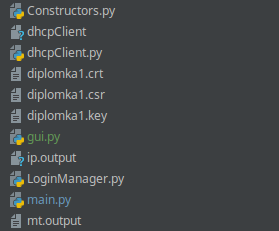
\includegraphics[scale=0.6]{../text/loginFiles.png}
\caption{Zoznam základných konfiguračných súborov}
\label{fig:filesLogin}
\end{figure} 
\subsection{Súbor centralControl}
\label{sec:central}
V súbore centrolControl sa popisuje spôsob hromadnej obsluhy mikrotikov na základe protokolu mactelnet. Pozostáva z metód:
\begin{itemize}
\item \textit{konštruktor} - pozostáva zužívateľských mien a hesiel, heslá v premennej credentials sú uložené ako slovník v podobe IP adresa: heslo
\item \textit{listMikrotikDevices()} - metóda vráti zoznam MAC a IP adries nájdených mikrotikov, uloží ich do súboru, a finálny výstup predstavuje list MAC adries
\item \textit{addCredentials()} - metóda pridíva heslo k užívateľskému účtu do slovníku, štandardnéužívateľské meno sa používa admin, ale tiež sa môže použiť aj iné užívateľské meno pri volaní metódy
\item \textit{loginSSH()}- metóda je použitá na hromadné prihlásenie pomoocu protokolu SSH na mikrotiky, používa sa tu pritom knižnica pexpect a jej subkižnica pxssh, jej vstupné parametre sp IP adresa serveru, užívateľské meno a heslo 
\end{itemize}
\begin{sexylisting}{Konštruktor súboru}
 def __init__(self, login):
        self.username = login
        self.credentials = {
            "192.168.1.1": "admin",
            "192.168.2.1": ""
        }
\end{sexylisting}
\begin{sexylisting}{Meóda zobrazenia mikrotikov}
 def listMikrotikDevices(self):
   deviceList = []
   loadAddress = False
   os.system("mactelnet -l -t 20 2>&1 > mt.output")
    with open( "mt.output", "r" ) as file:
     for line in file:
      if loadAddress:
         address = line.split( )[0]
         deviceList.append( address )
      else:
         header = line.split( )
         if len( header ) > 1:
            if "IP" in header[0]:
              loadAddress = True
         for i in deviceList:
           print(i)
  return deviceList
\end{sexylisting}
\begin{sexylisting}{Metóda pridania užívateľských mien a hesiel}
 def addCredentials(self, login="admin"):
   server_list = self.listMikrotikDevices()
   print( server_list )
   for server in server_list:
   try:
    password = self.credentials[server]
    except KeyError:
    password = input( "Please eneter the 
    password for " + server + ":" )
    self.credentials[server] = password
    return server_list
\end{sexylisting}
\begin{sexylisting}{Metóda hromadného prihlásenia pomocou protokolu SSH}
def loginSSH(self, server,login, password):
 from pexpect import pxssh, spawn, expect
 import getpass
 for server in self.credentials:
 try:
  connect = pxssh.pxssh( )
  server = self.credentials
  login = 'admin'
  password = self.credentials[server]
  port = 22
  connect.login( server, login, password )
  commands = pxssh.spawn( )
  time.sleep( 10 )
 except pxssh.ExceptionPxssh as e:
  print( "Error" )
  print( str( e ) )
\end{sexylisting}
\subsection{Súbor Constructors}
Súbor predstavuje zoznam konštruktorov pre konkrétne naprogramované API moduly pomocou knižnice tikapy. V úvode konštruktoru sú popísané importy jednotlivých modulov a submodulov pre konfiguráciu mikrotiku za pomoci API. \\
Následne je vytvorená trieda Mikrotik, ktorá zahŕňa všetky konštruktory spoločne s ich vstupnými parametrami, ktoré sú adresa,užívateľské meno a heslo. 
\begin{figure}[H]
\centering
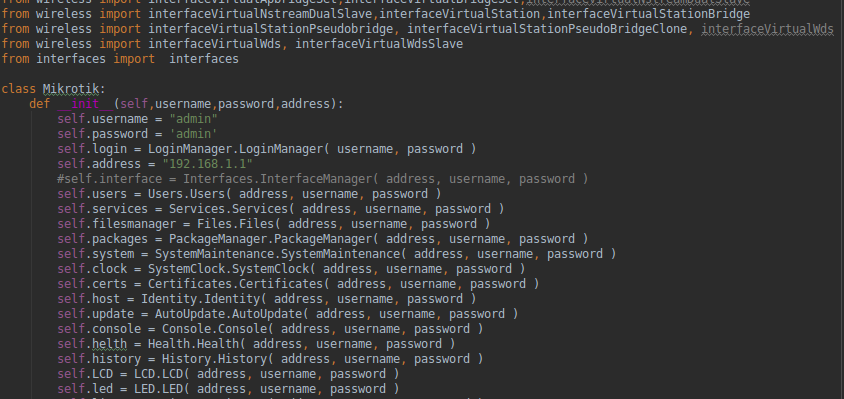
\includegraphics[scale=0.5]{../text/constructors.png}
\caption{Ukážka konštruktorov projektu}
\label{fig:constructors}
\end{figure} 
\subsection{Súbor dhcpClient}
V tomto súbore sa nachádza základná konfigurácia mikrotiku po pripojení naň. Obsahuje triedu basicConfig, ktorá pozostáva z dvoch metód.\\
V konštruktore sa nastaví rozhranie, na ktorom sa má adresa nastaviť, IP adresa/subnet a MAC adresa na pripojenie na mikrotik pomocu protokolu mactelnet.\\
\begin{sexylisting}{Trieda basicConfig}
class basicCOnfig:
    def __init__(self,interface,mac,ip):
        self.interface = interface
        self.mac = mac
        self.ip = ip
\end{sexylisting}
Prvá metóda \textit{dhcp()}, ktorej vstupné parametre sú užívateľské meno a heslo. Pozostáva z prihlásenia na mikrotik, a nastavenia Dynamic Host Client Protocol (DHCP) klienta na rozhraní, ktoré sa definuje pri volaní objektu v rámci konštruktoru.\\
\begin{sexylisting}{Metóda dhcp}
 def dhcp(self,username,password):
        child =pexpect.spawn('mactelnet '+self.mac)
        child.expect('Username:')
        child.sendline(username)
        child.expect('Password:')
        child.sendline(password)
        child.sendline('\r')
        try:
            child.expect('> ')
            child.sendline('ip dhcp-client add 
            interface='+self.interface+"\r")
            child.expect('> ')
            child.close()
        except:
            print("error")
            child.close()
        time.sleep(1)
\end{sexylisting}
Druhá metóda \textit{setAddress()}, ktorá bere ako vstupné parametre užívateľské meno a heslo nastaví statickú IP adresu na rozhraní definovanom v rámci konštruktoru.
\begin{sexylisting}{Metóda setAddress}
    def setAddress(self,username,password):
        child = pexpect.spawn( 'mactelnet '+ 
        self.mac )
        child.expect( 'Username:' )
        child.sendline( username )
        child.expect( 'Password:' )
        child.sendline( password )
        child.sendline( '\r' )
        try:
            child.expect( '> ' )
            child.sendline( 'ip address add address='
            +self.ip + " interface="
            +self.interface+"\r" )
            child.expect( '> ' )
            child.close()
        except:
            print( "error" )
            child.close()
        time.sleep( 1 )
\end{sexylisting}
\subsection{Súbor LoginManager}
Súbor LoginManager pozostáva z niekoľkých metód, tieto metódy majú podobnú štruktúru ako súbor centralConrol popisujúci v kapitole\ref{sec:central}.\\
Ako prvá popísaná časť je konštruktor, ktorý prijíma vstupné parametre užívateľské meno a heslo.\\
\begin{sexylisting}{Konštruktor súboru}
    def __init__(self, login,password):
        self.username = login
        self.pwd = password
\end{sexylisting}
Druhá metóda je metóda \textit{loginTelnet()},v rámci tejto metódy sa rieši prihlásenie na mikrotik pomocou protokolu telnet za použitia knižnice telnetlib. Vo vstupe metódy sa definuje premenná \textit{server_list}. Táto premenná je naplnená IP adresami mikrotikov v rámci súboru centralControl.\\
\begin{sexylisting}{Metóda loginTelnet}
    def loginTelnet(self, password, login="admin"):
        import telnetlib
        central = centralControl(login, password)
        server_list = central.listMikrotikDevices()
        print(server_list)
        for server in server_list:
            try:
                telnetcon = telnetlib.Telnet
                ( host=server, port=23 )
                telnetcon.read_until( b"Login: " )
                telnetcon.write( login.encode( )
                 + "\n" )
                telnetcon.read_until( b"Password: " )
                telnetcon.write( password.encode( )
                 + b"\n" )
                time.sleep( 10 )
                telnetcon.close( )
            except:
                print( "Cannot connect to 
                router via telnet" )
\end{sexylisting}
Ďalej sa tu nachádza metóda loginSSH(), táto metóda pracujúca podobne ako metoda loginTelnet() pracuje na základe protokolu SSH, na vstupe má server IP adresu, užívateľské meno  a heslo. \\
\begin{sexylisting}{Metóda loginSSH}
    def loginSSH(self, server,login, password):
        from pexpect import pxssh, spawn, expect
        import getpass
        try:
            connect = pxssh.pxssh( )
            server = '172.16.49.2'
            login = 'admin'
            password = 'admin'
            port = 22
            connect.login( server, login, 
            password )
            commands = pxssh.spawn( )
            time.sleep( 10 )
        except pxssh.ExceptionPxssh as e:
            print( "Error" )
            print( str( e ) )
\end{sexylisting}
Ďalšou metódou je metóda na vylistovanie všetkýchmikrotikov, táto metóda je bez vstupného parametru. Ako výstup je súbor mikrtik.output naplnený MAC adresami mikrotikov. 
\\
\begin{sexylisting}{Metóda listMikrotikDevices}
    def listMikrotikDevices(self):
        deviceList = []
        loadMacAddress = False
        os.system("mactelnet -l -t 20 
        2>&1 > mt.output")
        with open( "mt.output", "r" ) 
        as file:
            for line in file:
                if loadMacAddress:
                   macAddress = line.split( )[1]
                   deviceList.append( macAddress )
                else:
                    header = line.split( )
                    if len( header ) > 1:
                        if "IP" in header[0] 
                        and "MAC-Address" 
                        in header[1]:
                            loadMacAddress = True
        return deviceList
\end{sexylisting}
Poslednou metódou je metóda \textit{mactelnetLoginToSingleDevice()}, vďaka ktorej sa pripája pomocou protokolu mactelnet na jedno mikrotik zariadenie pomocou macadresy získanej z výstupu metódy \textit{listMikrotikDevices()} \textit{mikrotik.output}.
\begin{sexylisting}{Metóda mactelnetLoginToSingleDevice}
    def mactelnetLoginToSingleDevice(self, username, 
    password, address=None):
        deviceList = self.listMikrotikDevices()
        print( deviceList )
        if address:
            print('mactelnet {} -u {} -p {}'.format
            ( address, username, password ))
            os.system( 'mactelnet {} -u {} -p {}'.format
            ( address, username, password ) )
        elif deviceList:
            print( 'mactelnet {} -u {} -p {}'.format
            ( deviceList[0], username, password ) )
            os.system( 'mactelnet {} -u {} -p {}'.format
            ( deviceList[0], username, password ) )
        else:
            print("No device was found")
\end{sexylisting}
\section{Rozbor hlavnej časti backendu}
V rámci hlavnej konfiguračnej časti diplomovej práce, pre konfiguráciu backendu mikrotiku za pomoci porgramovacieho jazyka python som projekt rozdelil do niekoľkých častí:\begin{itemize}
\item \textbf{bridge} - táto časť obsahuje prvky konfiguácie, pridania, odstránenia, zapnutia, vypnutia možnosti bridgu na mikrotiku, konfigurácia existujúceho bridgu, zobrazenie zoznamu bridgov
\item  \textbf{capsman} - táto časť obsahuje konfiguráciu hromadnej obsluhy mikrotik úrístupových bodov a WiFi, profily, bezpečnosť, konfiguácie, povolené rýchlosti, zobrazenie zoznamu pripojených prvkov a ďalšie funkcie
\item \textbf{certs} - obsahuje certifikáty na pripojenie sa na mikrotik pomocou protokolu api-ssl
\item \textbf{Dude} - obsahuje popis konfigurácie ako nastaviť nástroj Dude klienta, ako nakonfigurovať Dude na vzdialený monitoring na Dude serveri, taktiež Dude server, a ďalšie možnosti
\item \textbf{exportToHtml} - časť predstavuje generovanie súboru na analýzu v podobe webovej stránky
\item \textbf{interfaces} - časť predstavuje konfiguráciu rozhraní na mikrotiku, tieto časti sú tiež popísané aj v iných zložkách ako napr. bridge. 4asť popisuje pridanie, odstránenie, zapnutie, vypnutie, konfiguráciu existujúcich rozhraní.
\item \textbf{IPv4} - rozsiahla časť, obsahuje konfiguráciu IP adries, firewallu, monitoringu, smerovania a ďalších nástrojov spadajúcich pod IP zložku na mikrotiku.
\item \textbf{IPv6} - pre zložku IPv6 platí to isté čo pre zložku IPv4, ale platí pre konfiguráciu na základe IPv6 adresného rozsahu
\item \textbf{KVM} - sekcia bude popisovať možnosti virtualizácie mikrotiku.
\item \textbf{log} - sekcia bude popisovať analýzu a konfiguráciu logu zariadenia
\item \textbf{makeSupportFile} - seckia bude popisovať vytvorenie súboru potrebného pre analýzu na mikrotik podpore
\item \textbf{mesh} - sekcia popisuje konfiguráciu tzv. mesh technológie, technológii podobne ako  v rámci časti bridge
\item \textbf{MPLS} - sekcia bude popisovať možnosti konfiurácie Multi Protocol Label Switching (MPLS), jej pridanie, odstránenie ,zapnutie, vypnutie, modifikácie a ďalšie funkcie.
\item \textbf{PPP} - sekcia bude popisovať konfiguráciu Point to Point Protocol (PPP) a ďalších možností Virtual Private Network (VPN) konfigurácie.
\item \textbf{Queues} - sekcia budep popisovať konfiguráciu sieťových front, možnosti front, typy front a ďalšie funkcie
\item \textbf{Radius} - sekcia bude popisovať nastavenie funkcie Radius - autentizačnej služby užívateľov , jeho modifikáciu, konfiguráciu a ďalšie funkcie.
\item \textbf{Routing} - sekcia bude popisovať možnosti dynamického smerovania, statické smerovanie bude popísané v rámci časti IPv4, dynamické smerovacie protokoly, ich konfigurácie, a ďalšie možnosti. 
\item \textbf{Switch} - sekcia bude popisovať konfiguráciu prepínača, niektoré mikrotiky sú typu SwitchOS a sú štandardne prepínač. Kofiguuráciu portov, trunkov, a ďalších funkcií. 
\item \textbf{System} - sekcia bude popisovať časť konfigurácie systémových nástrojov, ich funkcií a konfigurácie, a ďalších funkcií.
\item \textbf{Tools} - sekcia bude popisovať konfiguráciu mikrotik nástroj, a však nie všetky bolo možné odsimulovať v rámci konzolvej časti aplikácie, ich konfiguráciu, spustenie, riadenie a ďalšie funkcie. 
\item \textbf{Wireless} - sekcia bude obsahovať konfiguráciu bezdrátového rozhrania, moduly, módy, konfiguráciu, nastavenie, a ďalšie funkcie
\item \textbf{konfiguračné súbory mimo zložiek} - sekcia popísaná v kapitole  \ref{sec:popis1}, popisuje súbory na základnú konfiuráciu mikrotiku, nastavenie základnej konfigurácie.
\end{itemize}
Ukážka súborovej štruktúry je zobrazená na obrázku \ref{fig:structure}:
\begin{figure}[H]
\centering
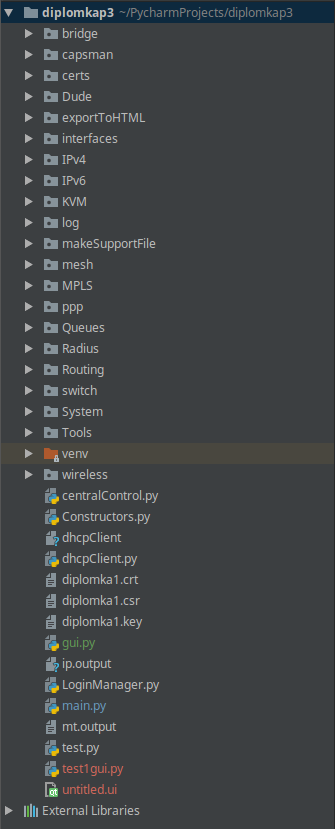
\includegraphics[scale=0.4]{../text/struktura.png}
\caption{Štruktúra projektu konzolovej časti projektu}
\label{fig:structure}
\end{figure} 
\chapter{Hlavná časť backendu}
Cieľom kapitoly je detailný popis backend časti aplikácie na správu mikrotikov. V jendotlivých podkapitolách bude popísaná každá zložka projektu diplomkap3.
\section{Zložka bridge}
